\paragraph{Tijdsduur}
Bij het afspelen van audio of video is er niet echt een meting om te doen. 
De audio of video dat afspeelt is ofwel spelend ofwel niet spelend.
Daarom wordt er enkel gekeken naar het CPU en geheugen gebruik tijdens 
het afspelen van audio en video.

\paragraph{CPU \& geheugen}
\begin{figure}[H]
    \centering
    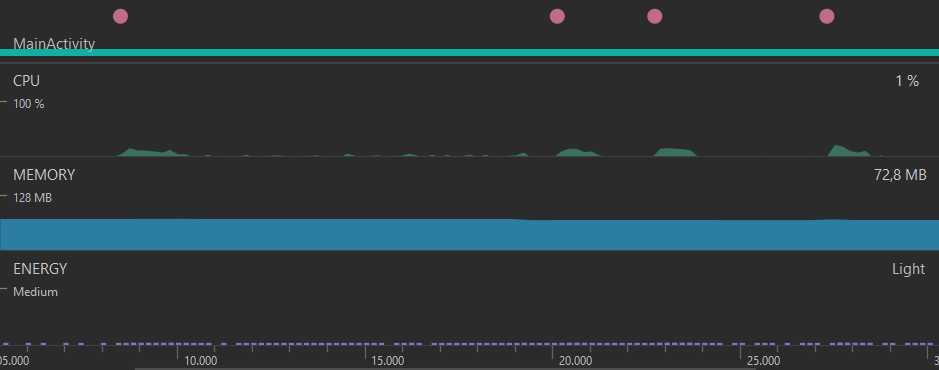
\includegraphics[height=0.3\textheight]{mediaPerformantieNative.png}
    \caption{Overzicht CPU en geheugen gebruik tijdens het afspelen van audie en video bij Android.}
\end{figure}
De eerste twee klik events zijn voor het starten en pauzeren van de video. Op de grafiek 
is te zien dat het CPU gebruik stijgt tot 17\% en daarna afwzakt naar een wisselend gebruik 
van 0 - 7\%. Bij het pauzeren van de video stijgt het CPU gebruik tot 16\% en daarna
zakt het terug naar 0\%. Het geheugen gebruik tijdens het afspelen van de video komt overeen 
met het geheugen gebruik bij het inactief zijn van de applicatie. Er is dus geen verschil in
geheugen gebruik bij het afspelen van de video.
\\\\
De laatste twee klik events zijn voor het starten en pauzeren van de audio. Op de grafiek
is te zien dat het CPU gebruik opnieuw stijgt tot 17\%. In tegenstelling tot de video is 
er geen wisselend CPU gebruik. Het CPU gebruik blijft constant rond 0 - 1\%. Bij het pauzeren
van de audio stijgt het CPU gebruik tot 23\% en zakt daarna terug naar 0\%. En net zoals bij de 
video is er geen verschil in geheugen gebruik bij het afspelen van de audio. Het geheugen gebruik
tijdens het afspelen van de audio komt opnieuw overeen met het geheugen gebruik bij het inactief zijn van
de applicatie.